\documentclass[12pt]{article}
\usepackage[utf8]{inputenc}
\usepackage[finnish]{babel}
\usepackage{graphicx}
\title{Aineopintojen harjoitustyö: Tietokantasovellus\\Dokumentaatio}
\author{Sandra Luhtaniemi\\013734363}
\begin{document}
\maketitle
Harjoitustyön aiheena on lankatietokanta. Tietokannan tarkoitus on tarjota käyttäjälleen väline, jolla pitää kirjaa omistamistaan eri käsityölangoista, näiden materiaalista, paksuudesta ja määrästä. Käyttäjä voi esimerkiksi kohdatessaan kiinnostavan neuleohjeen, hakea ohjeessa mainitun langan ominaisuuksien perusteella tietokannasta ne langat, joilla työ olisi mahdollista toteuttaa, sekä tarkistaa, onko hänellä sitä riittävä määrä. Käyttäjä voi myös muilla perusteilla etsiä tietokannasta lankoja, esimerkiksi vaikkapa kaikki sukkalangat. Käyttäjä voi lisätä tietokantaan uudet lankahankintansa, poistaa langan, tai päivittää sen määrän käytettyään jotakin lankaa. Järjestelmän tavoitteena on helpottaa käsitöiden suunnittelua ja vähentää turhia lankahankintoja.
\\
\ \\
\textbf{Käyttötapaukset}\\ 
Käyttäjäryhmät:\\
Tietokannalla on vain yksi käyttäjäryhmä. Käyttäjän on rekisteröidyttävä päästäkseen käyttämään tietokantaa. Tämän jälkeen hän voi lisätä tietokantaan lankojaan ja tarkastella tai suorittaa hakuja omistamistaan langoista. 
\\ \ \\
Käyttäjän käyttötapaukset\\
Rekisteröityminen: Käyttäjä luo ensimmäisellä käyttökerralla itselleen käyttäjätunnuksen ja salasanan.
\\ \ \\
Langan lisääminen: Käyttäjä lisää tietokantaan uuden langan
\\ \ \\
Langan poistaminen: Käyttäjä poistaa tietokannasta langan, jonka on käyttänyt loppuun.
\\ \ \\
Langan määrän päivittäminen: Käyttäjä päivittää langan määrän käytettyään siitä osan.
\\ \ \\
Lankojen tarkastelu: Käyttäjä tarkastelee listaa omistamistaan langoista.
\\ \ \\
Haku ominaisuuden perusteella: Käyttäjä hakee tietokannasta kaikki jollakin ominaisuudella varustetut langat.
\\ \ \\
Omien tietojen muuttaminen: Käyttäjä muuttaa omia tietojaan, esimerkiksi salasanaansa tai nimeään.
\\ \ \\
\begin{figure}[!h]
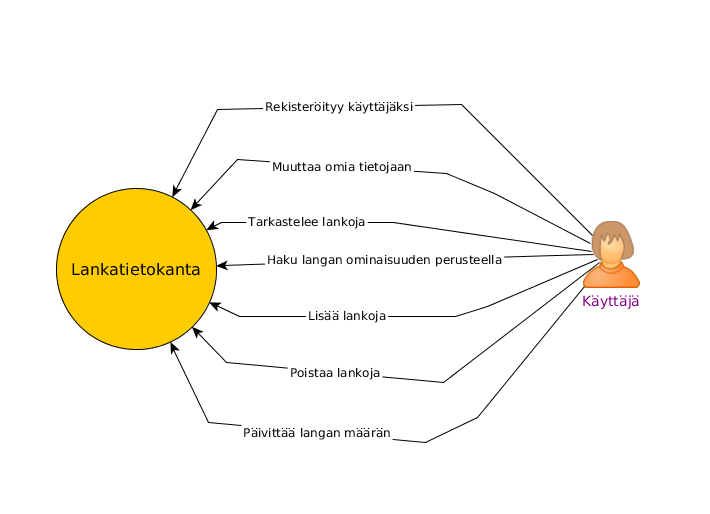
\includegraphics[scale=0.5]{sidosryhmakaavio.png}
\caption{Sidosryhmäkaavio}
\end{figure}
\begin{figure}
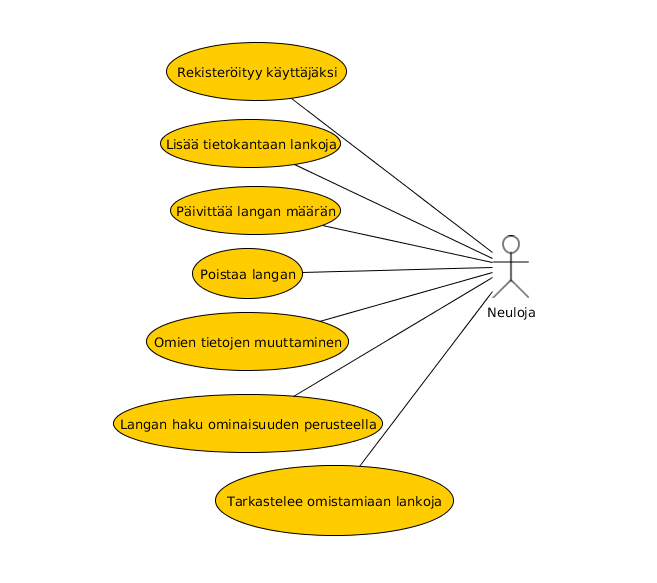
\includegraphics[scale=0.5]{kayttotapaukset.png}
\caption{Käyttötapauskaavio}
\end{figure}
\end{document}
